\chapter{Diskussion der Messergebnisse}

Durch den Laborversuch konnten erste Erfahrungen mit der Konfiguration
von IPv6-\acsp{LAN} gesammelt werden. Dar�ber hinaus konnte das Wissen �ber die
Konfiguration von Cisco-Hardware (Switches und Router) vertieft werden.
\newline
Besonders hervorzuheben sind die Multicast-Adressen die Teil des Versuchs sind.
Um mehr dar�ber zu erfahren und die Theorien aus \ref{multi} zu best�tigen,
wird im Folgenden ein weiteres Szenario �berpr�ft.

\section{NDP und Solicited-Node Multicast-Adressen}
Solicited-Node Multicast-Adressen (siehe \ref{solicited}) waren bisher kein
Gegenstand des Studiums.
Zum Verst�ndnis diente der \acs{RFC} 4291, \citetitle{RFC4291}. Dar�ber hinaus
wurde zur Veranschaulichung der Simulation Mode des Packet Tracers genutzt.
\clearpage
\subsection{Beispielszenario}
Ein Paket wird von PC1 zu PC3 gesendet. Hierbei werden \acs{ICMP}v6- und
\acs{NDP}-Pakete gefiltert. Die Pakete werden analysiert.

\begin{figure}[!htbp]
  \centering
     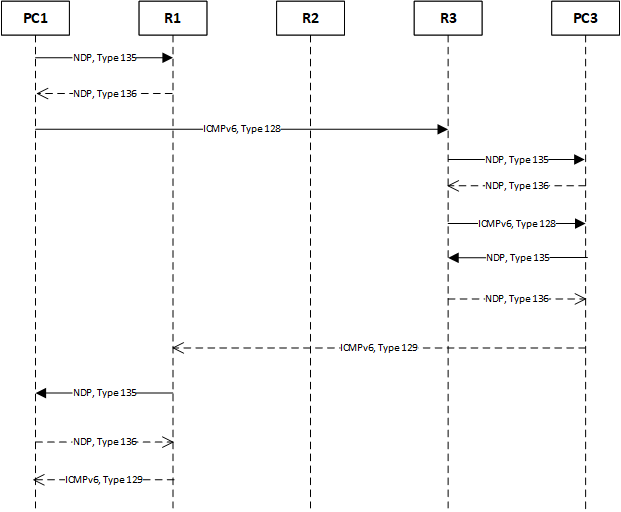
\includegraphics[width=\linewidth]{Graphics/ndp.PNG}
  \caption{Ping von PC1 zu PC3}
  \label{fig:aufbau}
\end{figure}
Zun�chst wird eine NDP-Anfrage (Neighbor-Solicitation-Nachricht) mit Message
Type 135 zum Router 1 gesendet. Ziel ist die Solicited-Node Multicast-Adresse
von Router 1 (FF02::1:FF00:1). Router 1 antwortet mit einer
Neighbor-Advertisement-Nachricht (Message Type 136).
\newline
Danach wird der Echo-Request (Message Type 128) von PC1 zu PC3 gesendet.
Sobald die Anfrage Router 3 erreicht, wird eine Neighbor-Solicitation-Nachricht
von Router 3 zu PC3 gesendet. Ziel dieser Nachricht ist die Adresse
FF02::1:FF00:F. Diese entspricht der Solicited-Node Multicast-Adresse von PC3.
\newline
Nach der darauf folgenden Neighbor-Advertisement-Nachricht von PC3 zu Router 3
wird der Echo Request fortgesetzt und erricht PC3.
\newline
Es folgt ein weiteres NDP-Paket mit Message Type 135 von PC3 zu Router 3
(Zieladresse: FF02::1:FF00:3).
Dieser antwortet wieder mit einem NDP-Paket des Typs 136.
\newline
Im Anschluss beginnt die Echo Reply Nachricht (Type 129) von PC3. Bei Router 1
angekommen, wird erneut ein NDP-Paket versandt. Ziel der Neighbor-Solicitation-Nachricht ist
PC1 (Zieladresse: FF02::1:FF00:F), welcher mit einer
Neighbor-Advertisement-Nachricht antwortet.
\newline
Im letzten Schritt wird der Echo Request von Router 1 zu PC1 weitergeleitet.
\newline
\newline
Dieses Szenario veranschaulicht, wie NDP die Solicited-Node Multicast-Adressen
nutzt. Die ICMPv6-Nachrichten verhalten sich �quivalent zu ICMP-Nachrichten bei
IPv4.
